% !TeX program = lualatex

\documentclass[tikz,border=10pt]{standalone}
\usepackage{tkz-graph}
\usepackage{amsmath,amssymb}
\usepackage{xcolor}
\usetikzlibrary{calc}
\usetikzlibrary{positioning, quotes}
\usetikzlibrary{arrows.meta}

\tikzset{mytext/.style = {font=\sffamily\bfseries, text=white},
        vertex/.style = {mytext, shape=circle, ball color = #1},
        number/.style = {mytext, draw, fill=red}}

\tikzset{vertex/.default = blue}

\tikzset{highlight/.style = {draw=yellow, very thick, densely dotted},
        highlight vertex/.style = {vertex, highlight},
        highlight number/.style = {number, highlight}}

\tikzset{bridge/.style = {thick ,  double=yellow, double distance= 1pt}}

\begin{document}

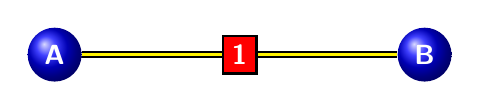
\begin{tikzpicture}
	\node [vertex] (A)  {A};
	\node [vertex, right = 4cm of A] (B)  {B};
	\draw (A) edge[bridge] node[number] {1} (B);
\end{tikzpicture}



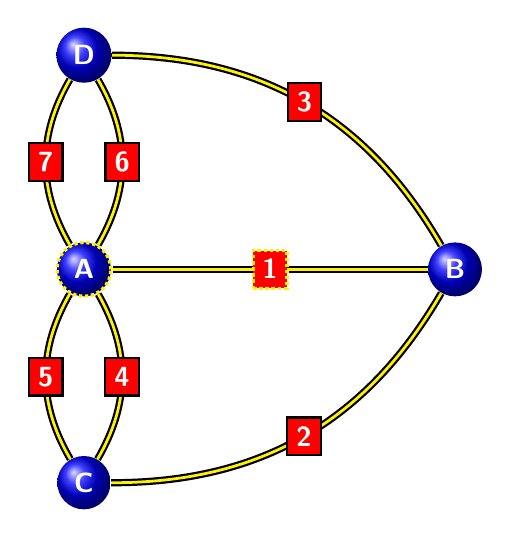
\begin{tikzpicture}
	\node [highlight vertex] (A) {A};
	\node [vertex, right = 4cm of A] (B) {B};
	\draw (A) edge[bridge] node[highlight number] {1}  (B);

	\node [vertex, below=2cm of A] (C)  {C};
	\node [vertex, above=2cm of A] (D) {D};

	\tikzset{bridge/.append style = {bend right}}

	\draw (C) edge [bridge]  node[number] {2} (B)
	(B) edge [bridge] node [number] {3} (D)
	(C) edge [bridge] node [number] {4} (A)
	(A) edge [bridge] node [number] {5} (C)
	(A) edge [bridge] node [number] {6} (D)
	(D) edge [bridge] node [number] {7} (A);
\end{tikzpicture}




\end{document}
